\chapter{Phase 1 FPix upgrade modules}

In chapter \ref{ch:cms}, a description of the CMS pixel detector used during the collection of the data sets used in this analysis, was presented. During the extended year-end technical stop (EYETS) 2017, the complete CMS pixel detector was replaced in order to support the full performance of the CMS experiment under the higher radiation conditions produced by the increasing instantaneous luminosity delivered  by the LHC accelerator. It also was designed to address and mitigate the identified weaknesses in the previous system.

In this chapter, a description of the upgraded detector will be presented. Emphasis will be put on the contributions made by the University of Nebraska - Lincoln (UNL) HEP group, which consisted of the assembly of about 600 of the modules that make up the phase 1 upgraded forward pixel detector (FPix); in particular, the gluing and encapsulation stages will be described in detail since they are my contributions. A complete description of the upgrade design and plans is presented in Reference \cite{tdr} which is the main source of the information contained in this section unless additional references are provided.   

\section{CMS pixel detector upgrade}

The previous pixel detector was designed to record efficiently and with high precision the first three space-points near the interaction region, in the range of $|\eta|<2.5$,  at a instantaneous luminosity of $1\times10^{34}$ cm$^{-2}$s$^{-1}$ and a bunch crossing each 25 ns. An average pileup of about 25 simultaneous overlapping events is expected. The increasing luminosity would affects the performance of the detector reducing track reconstruction efficiency, and increasing the data loses caused by the degradation of the readout system; furthermore, if the LHC runs with 50 ns bunch spacing at twice the luminosity, then the data losses would increase almost exponentially, to losses of 50\% for the innermost layer. An illustration of the foreseen reduced performance in tracking efficiency and data loss is shown in Figure \ref{fig:reduced_performance} in the case of simulated \ttbar events at instantaneous luminosities up to $2\times10^{34}$ cm$^{-2}$s$^{-1}$ with 25 ns and 50 ns bunch spacing. The increasing fake rate is also showed. In conclusion, the prevoius pixel detector was not able to perform efficiently under the new luminosity, pileup, radiation, and running conditions.  

\begin{figure}[!h]
\centering
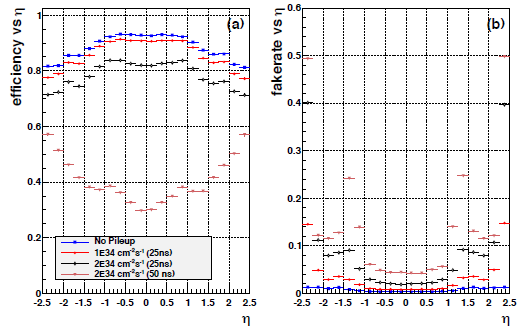
\includegraphics[width=0.9\textwidth]{pixel/reducedperformance2}
%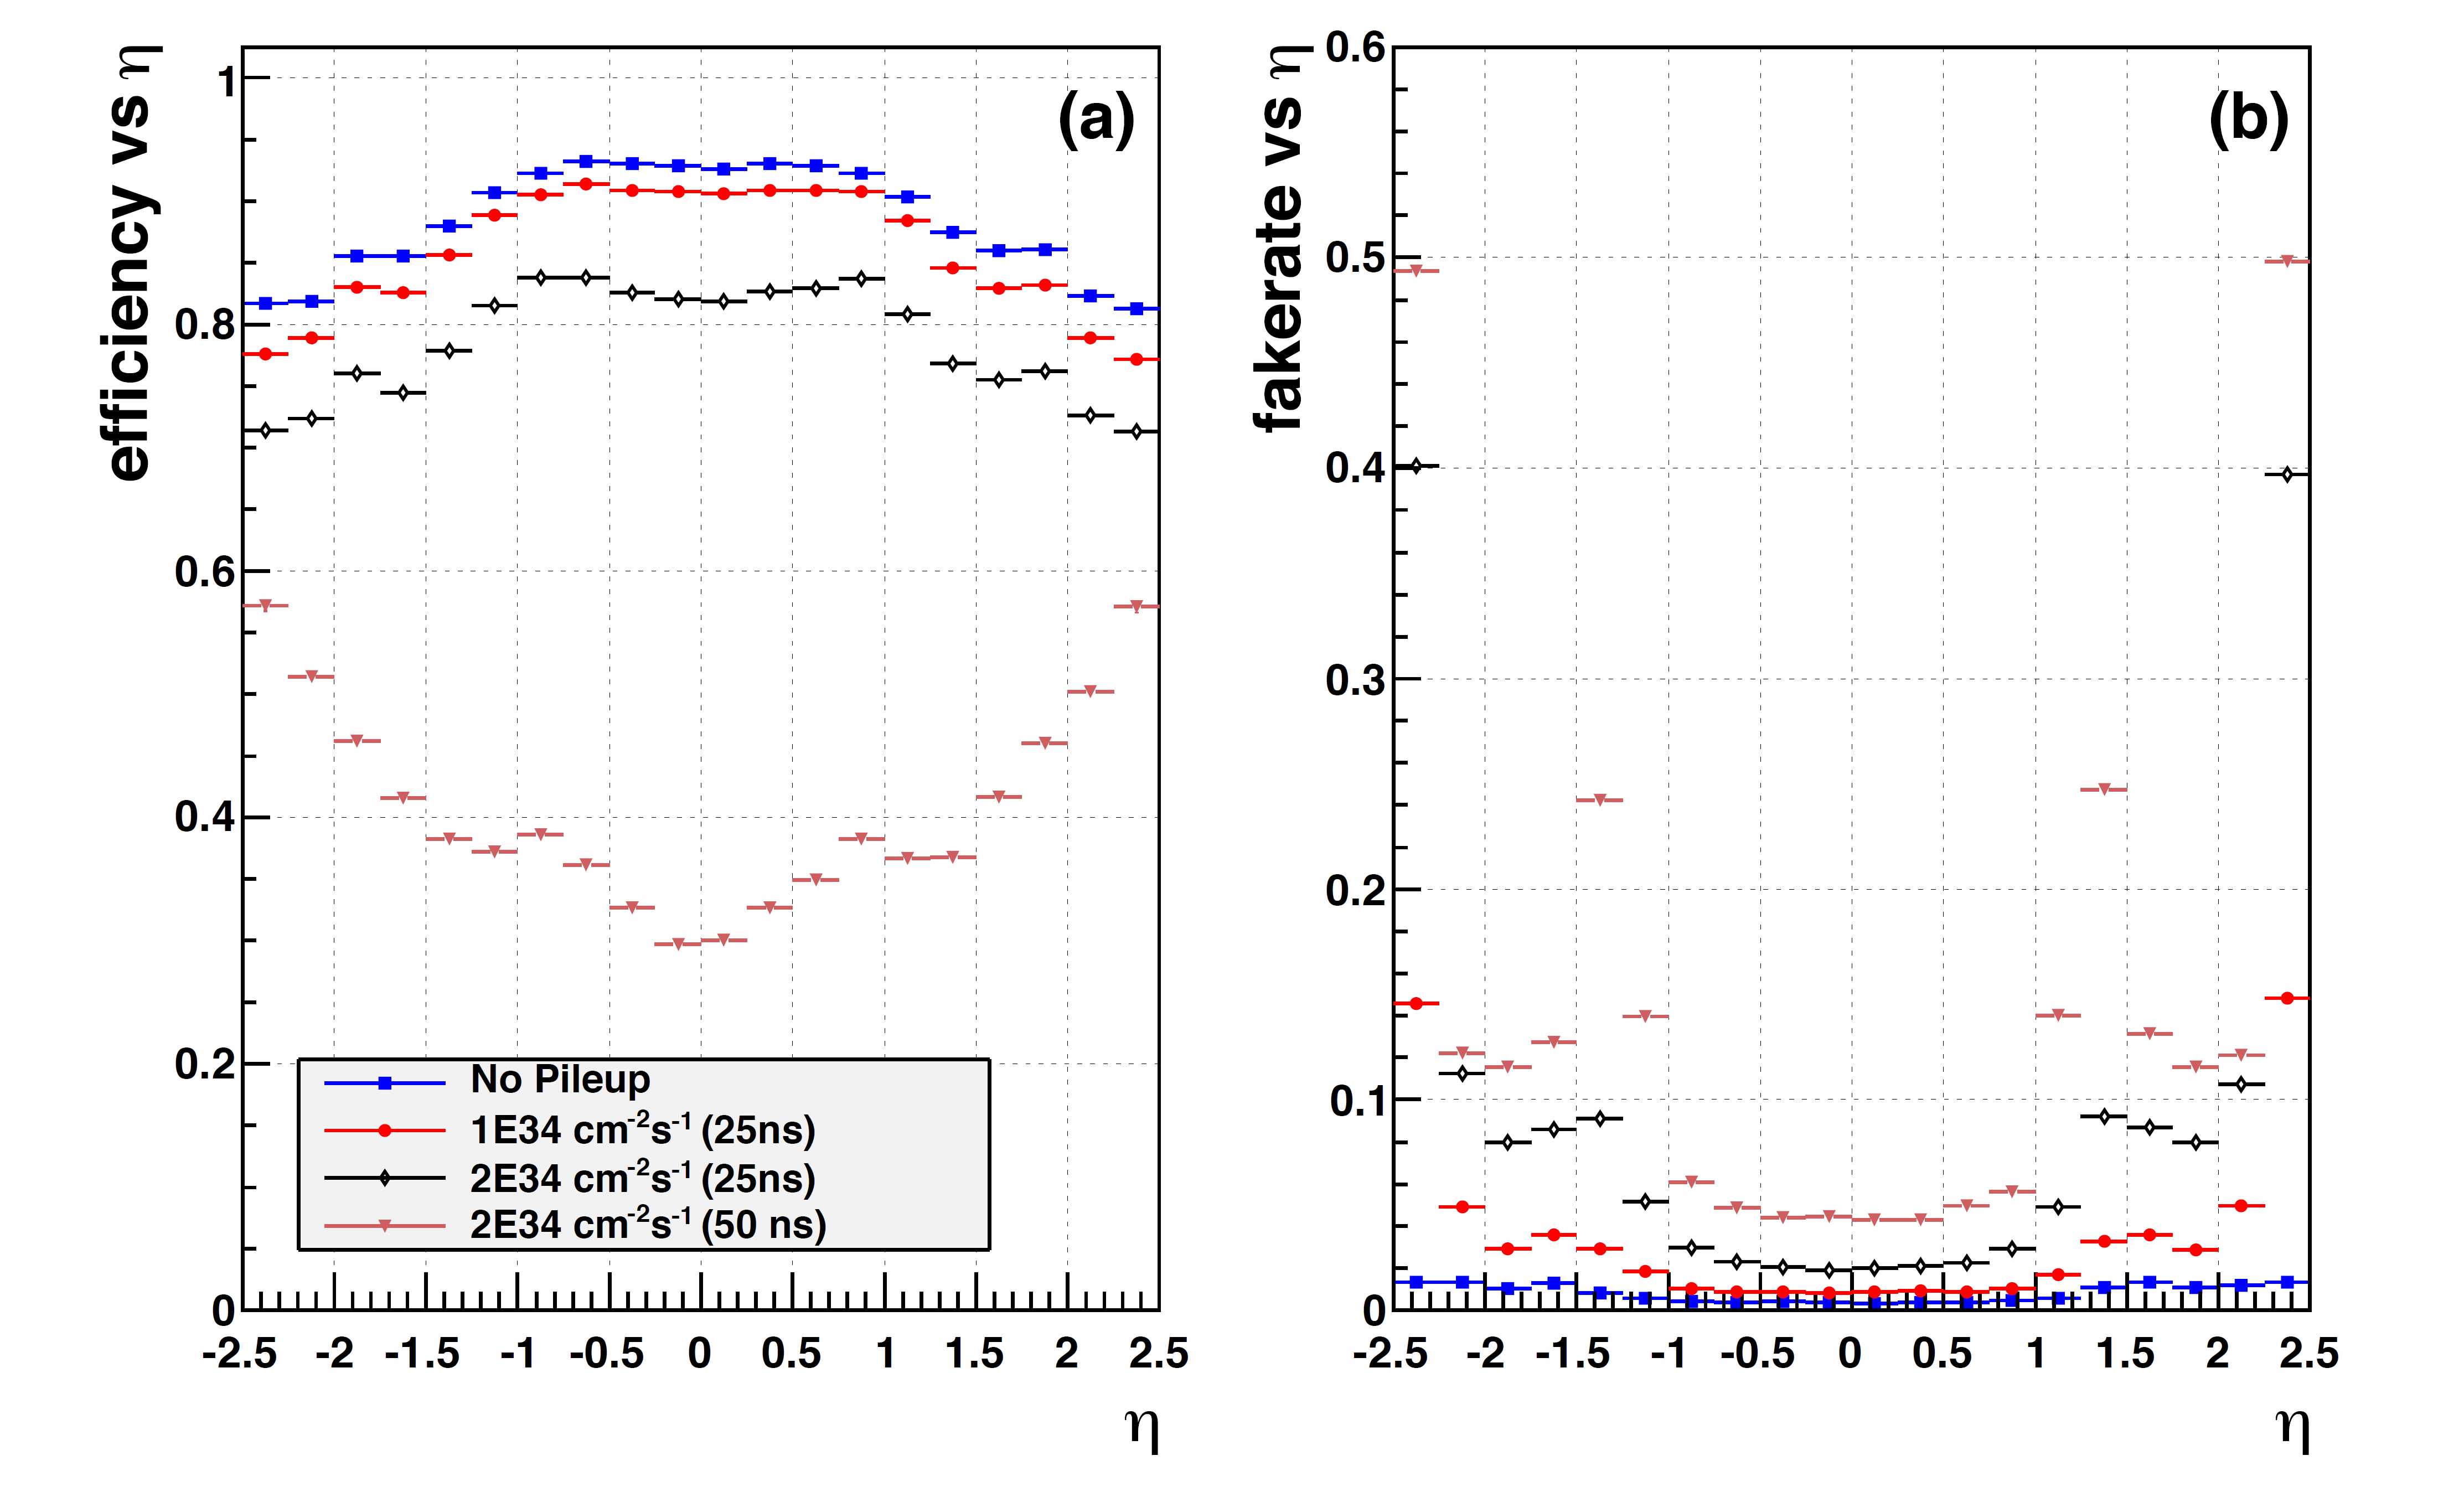
\includegraphics[width=0.9\textwidth]{pixel/reducedperformance}
\caption[Expected performance of the previous pixel detector in simulated \ttbar events.]{Expected performance of the previous pixel detector in simulated \ttbar events: a) efficiency; b) fake rate. Conventions are the same for both plots, considering zero pileup (blue squares), average pileup of 25 (red dots), average pileup of 50 (black diamonds), and average pileup of 100 (magenta triangles).}\label{fig:reduced_performance}
\end{figure}

The present system is designed to offer high performance under these new operational conditions; it is composed of four-layers/three-disks, low mass silicon pixel detectors providing a high performance tracking in the high luminosity environment. The design was leaded by the following requirements\footnote{Taken literally from the technical design report.} 
\bit
\item In running with 50 or more pile-up, maintain the high efficiencies and low fake rates.
\item New pixel readout chip (ROC) to minimize data loss due to latencies and limited buffering in high luminosity running.
\item Minimize degradation due to radiation damage.
\item Optimized detector layout for 4-pixel-hit coverage over the \etac range with minimal innermost layer radius improving pattern recognition and track reconstruction.
\item To reduce material, adopt two-phase $CO_2$ cooling and light-weight mechanical support, moving the electronic boards and connections out of the tracking volume.
\item To reuse the current patch panel and off-detector services, cooling pipes, cables and fibers, adopt DC-DC power converters and higher bandwidth electronics.
\item Reduce number of module types and interfaces simplifying production and maintenance.
\item New smaller diameter beam pipe to accommodate the placement of the inner pixel layer closer to the interaction region.
\eit

The upgraded detector is expected to provide higher efficiencies, lower fake rates, lower dead-time/data-loss, and an extended lifetime of the detector, which translate in better muon ID, b-tagging, photon/electron ID, and tau reconstruction, in both HLT and offline levels. No details about the performance of the current pixel detector are given here since that matter falls beyond the purpose of this document; however, it is documented in Reference\cite{pixel_performance}.

Figure \ref{fig:new_pix} shows the layout of the upgraded pixel detector. The old 3-layer barrel (BPIX), 2-disk endcap (FPIX) system is replaced with a 4-layer barrel, 3-disk endcap system. The additional barrel layer and forward disk provide redundancy for the track pattern recognition and reconstruction.

\begin{figure}[!h]
\centering
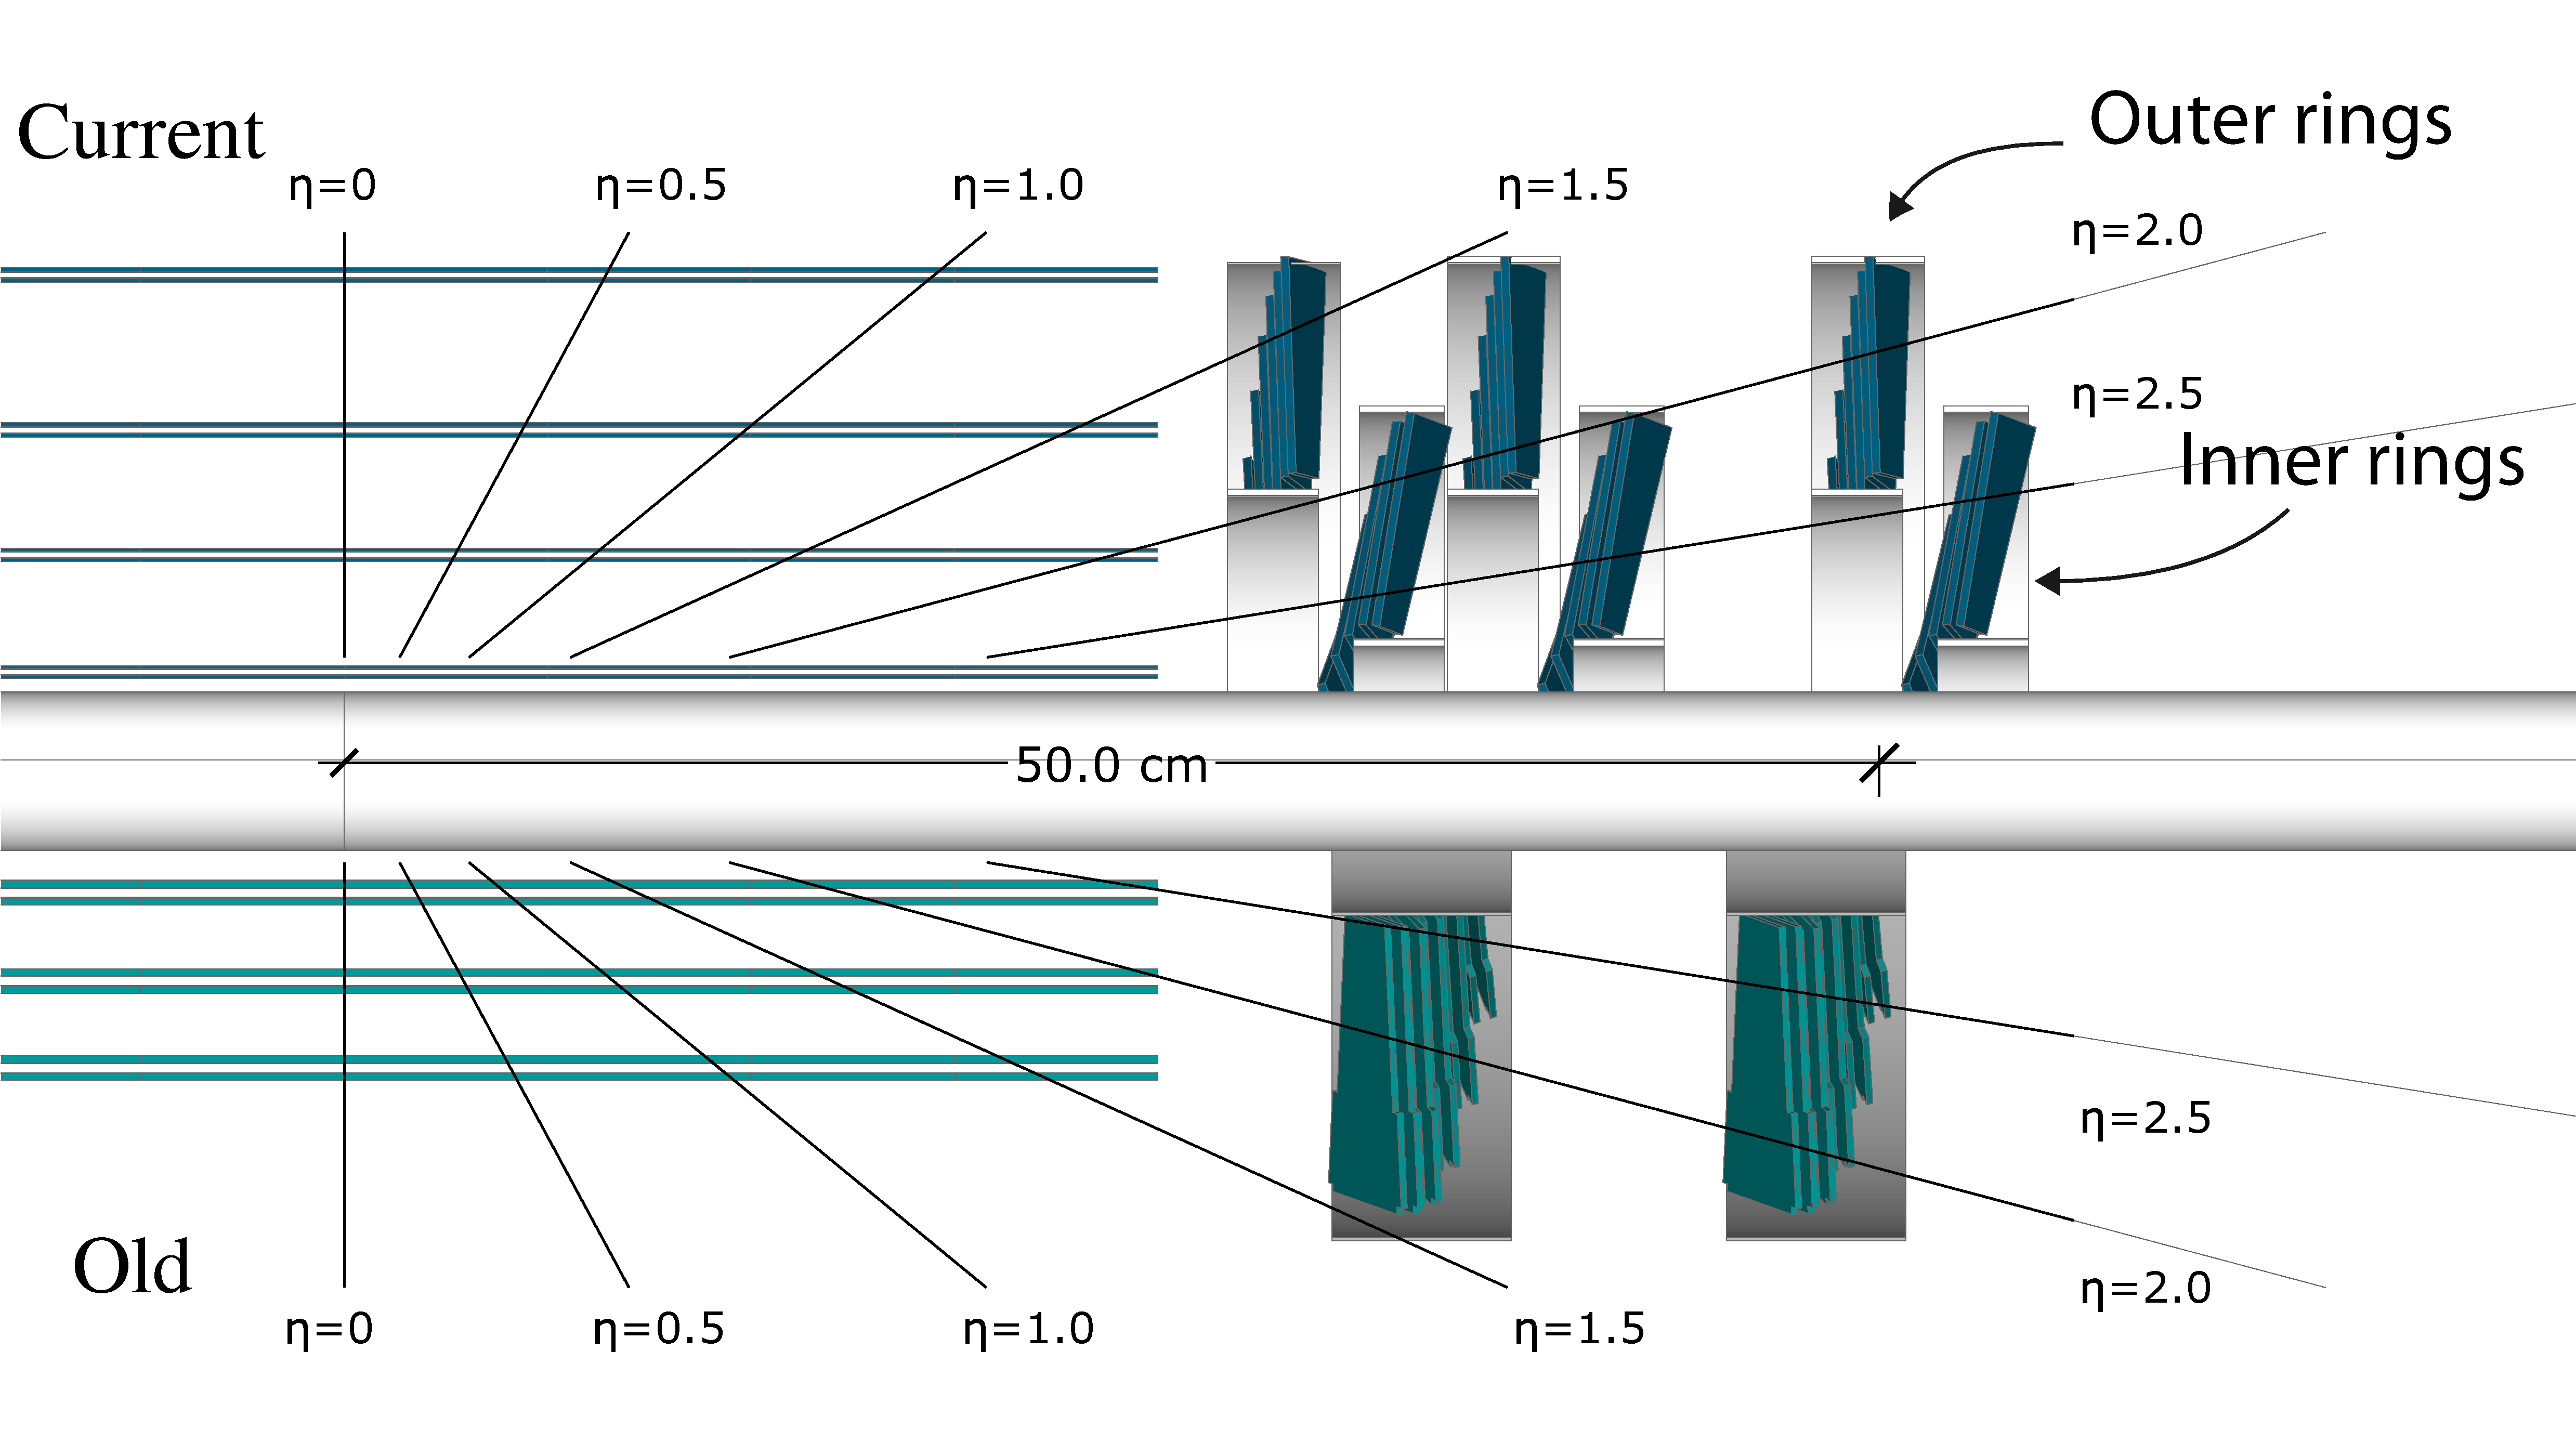
\includegraphics[width=0.6\textwidth]{fpix1.pdf}
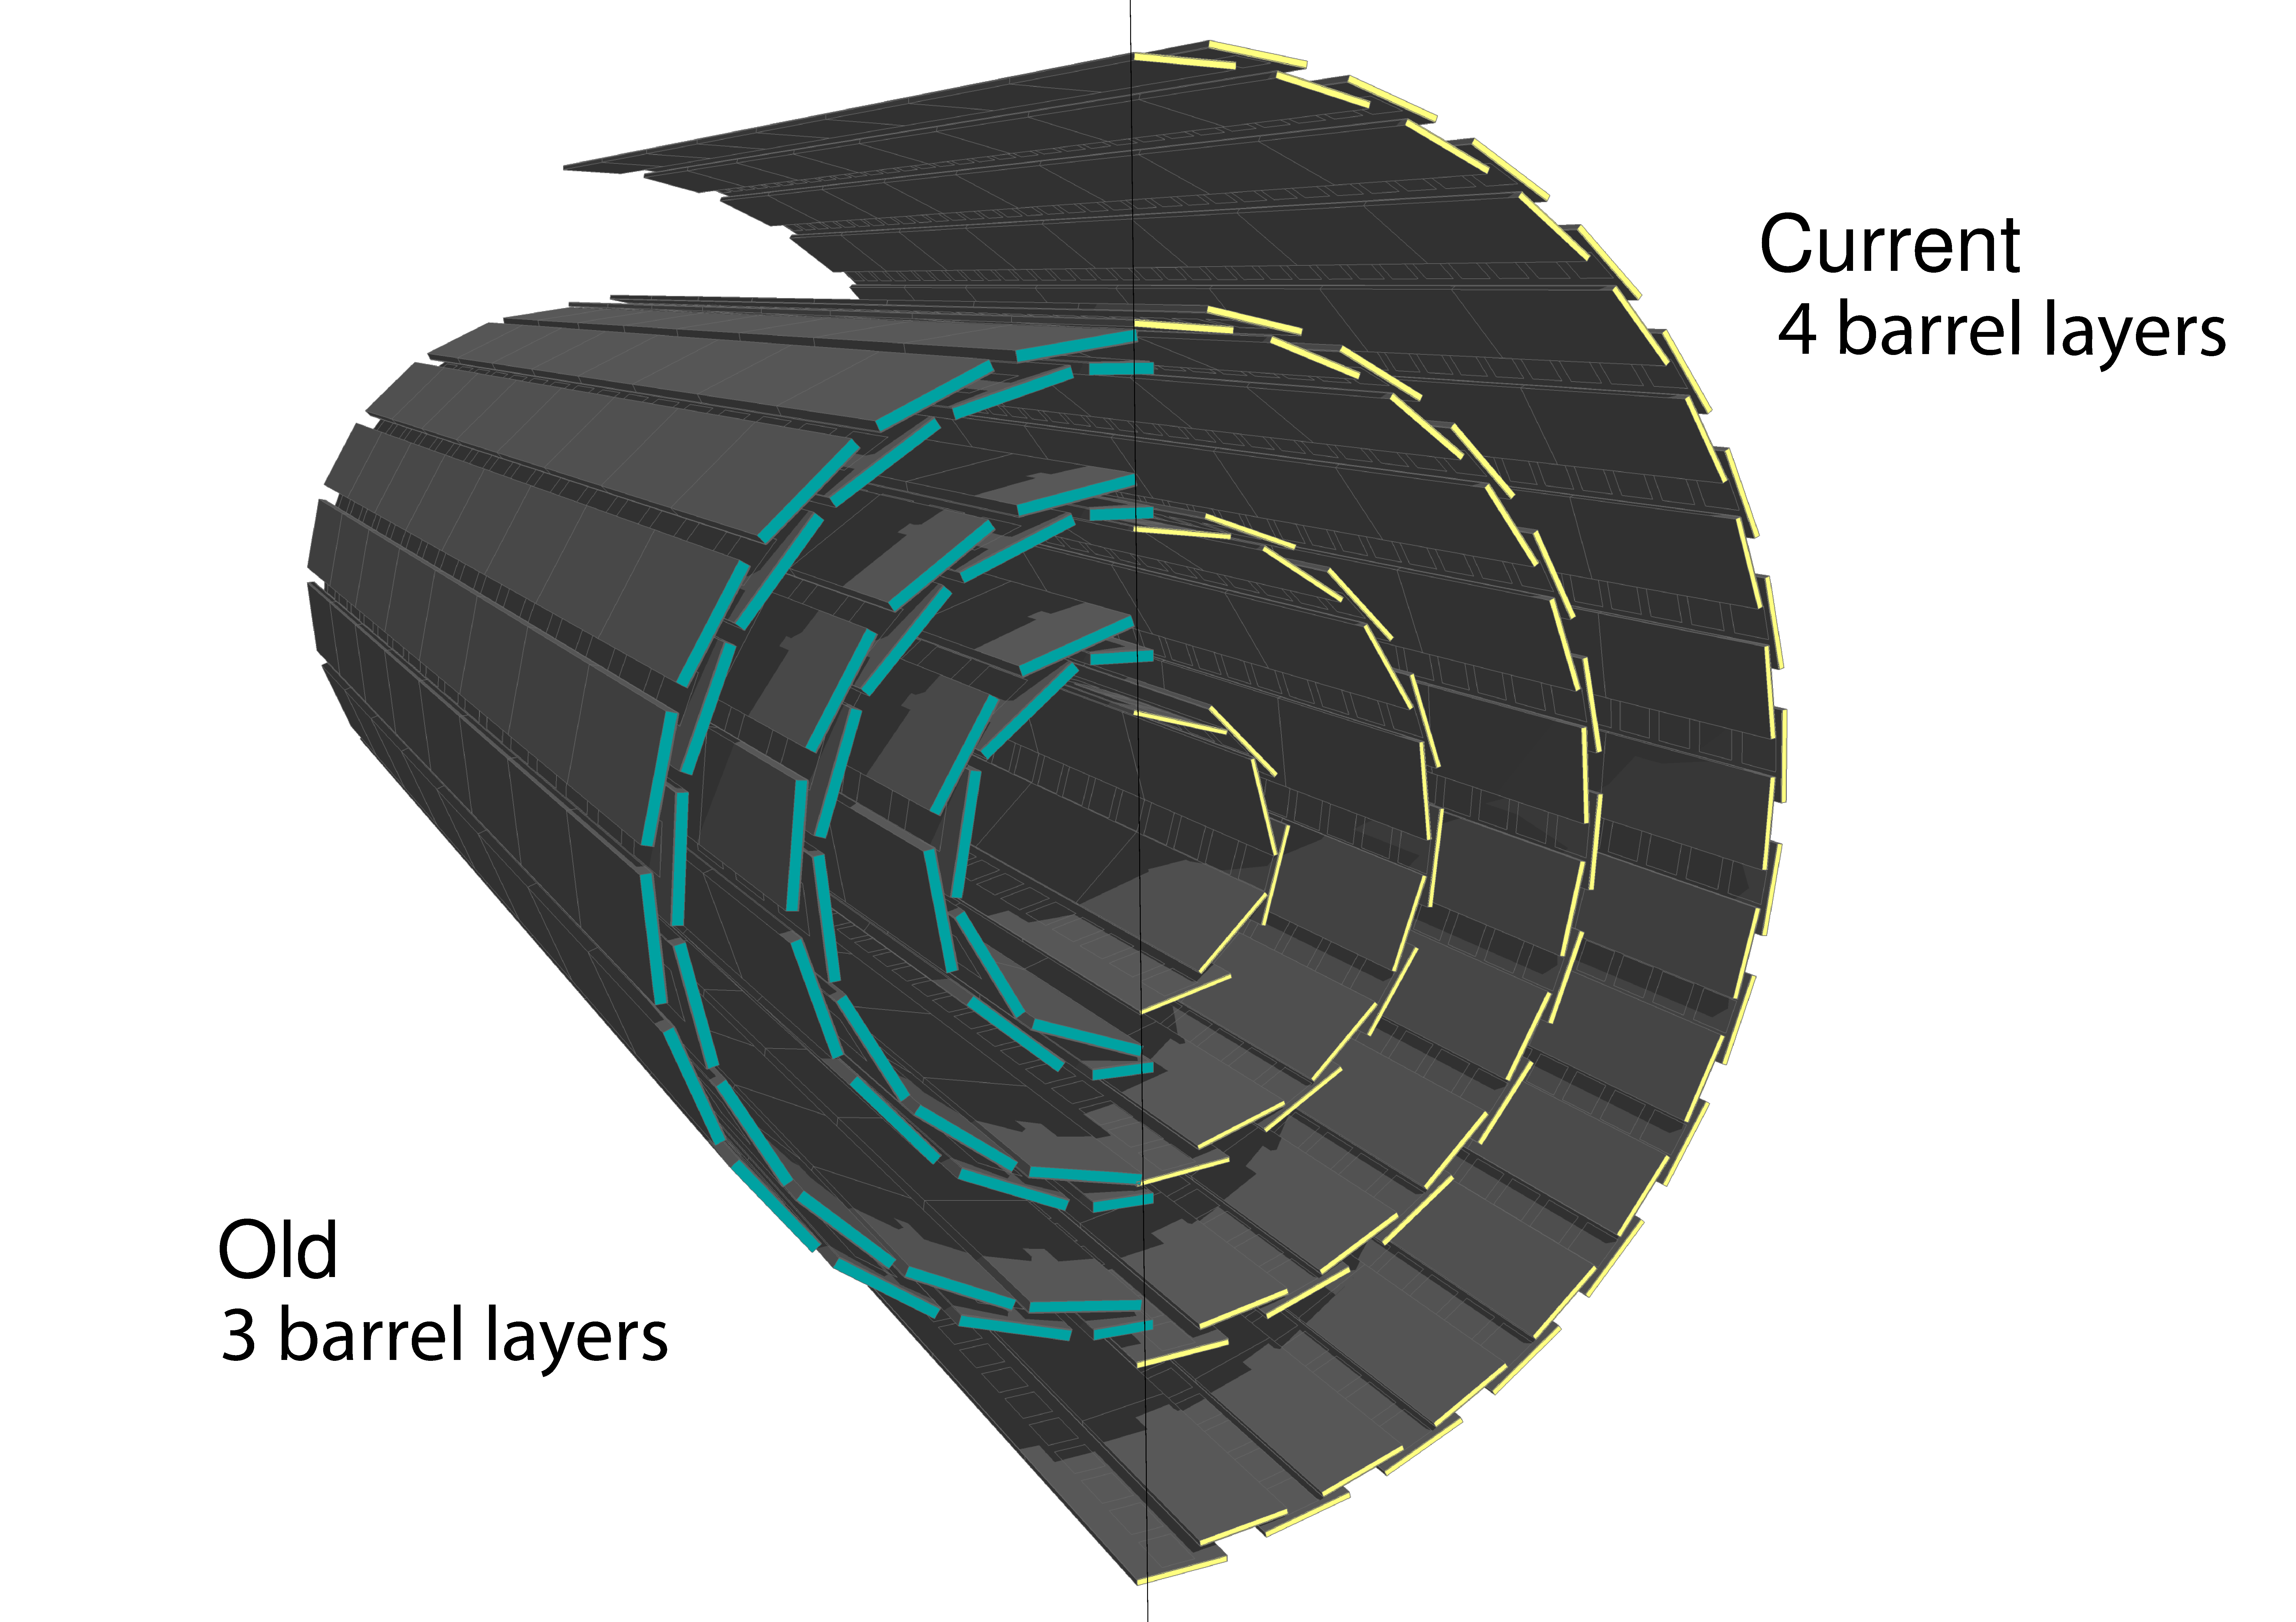
\includegraphics[width=0.39\textwidth]{bpix1.pdf}
\caption[Layout of the upgraded and old pixel detectors.]{Layout comparing the different layers and disks in the current and old pixel detectors.}\label{fig:new_pix}
\end{figure}

\section{Phase 1 FPix upgrade}

The Phase 1 upgraded FPix system is composed of three disks in each endcap, located at each end of the barrel detector, with a radial coverage ranging from 4.5 to 16.1 cm. The first disk is located along the beam line at 29.1 cm from the IP; the second and third disks are located at 39.6 cm and 51.6 cm from the IP; each disk consists of two half disks. Some of the main features of the upgraded FPix System are:
\bit
\item Pixel size: $100 \times 150$ $\mu$m 
\item Only one type of modules: 2x8 ROC modules
\item Modules oriented radially to improve resolution in $r-\phi$.
\item Minimize the gap in 4-hit coverage between the end of the 4th-barrel layer and the forward-most disk.
\item All three identical disks on each side of the IP.
\eit

Figure \ref{fig:fpix_layout} shows a schematic structure of the FPix half disk; each half disk is composed of two sections, inner and outer, where the pixel modules are assembled.

\begin{figure}[!h]
  \centering
  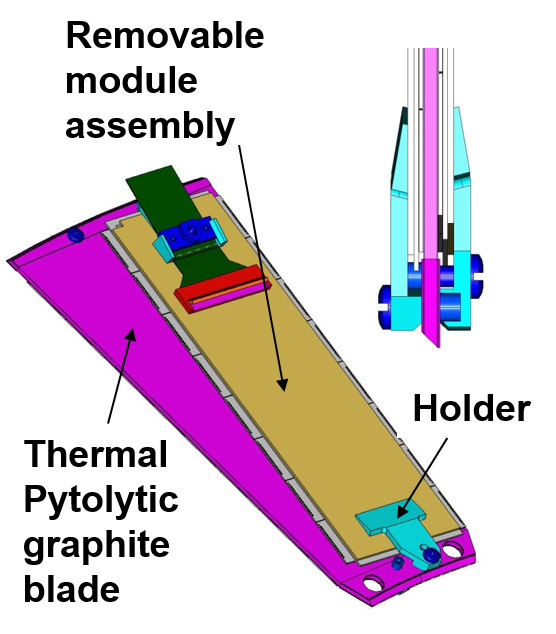
\includegraphics[width=0.32\textwidth]{pixel/module1}
  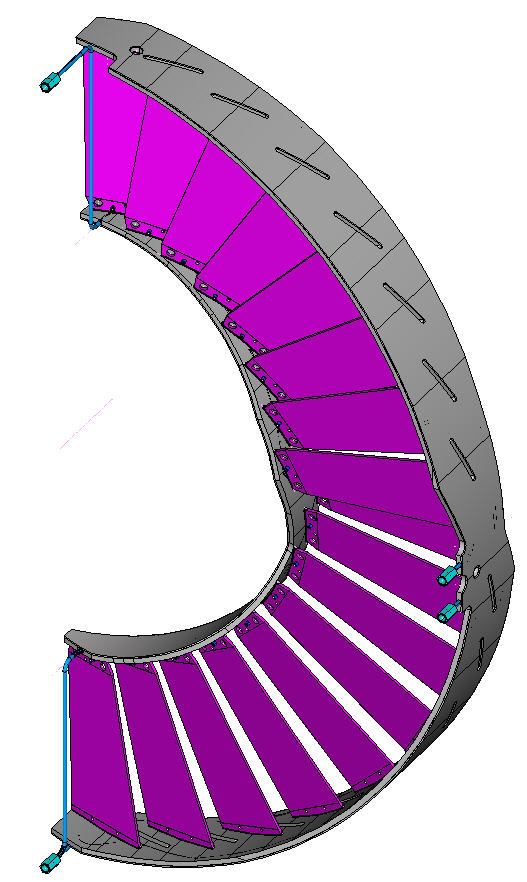
\includegraphics[width=0.32\textwidth]{pixel/half_disk_inner}
  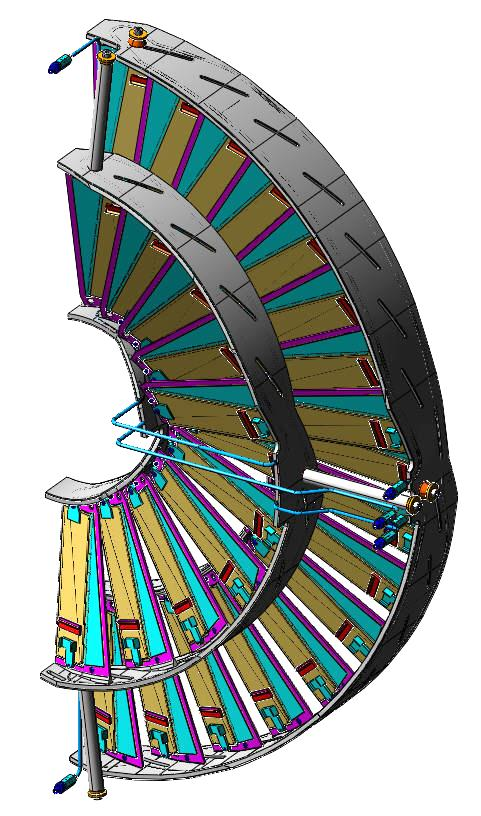
\includegraphics[width=0.32\textwidth]{pixel/half_disk}
\caption[FPix half disk design.]{FPix half disk design; FPix module (left) mounted on a blade, outer half disk (center), assembled half disk (right).}\label{fig:fpix_layout}
\end{figure}

In total, there are 56 modules (896 ROCs) per half-disk, 34 modules in the outer ring and 22 modules in the inner ring. The pixel modules are attached to the blades by a pair of module holders. Modules are designed to be removable and replaceable without disassembling the half-disks; thus those modules that suffer failure or degradation can be easily replaced during an annual technical stop.

Blades on the outer assembly are rotated by 20$^o$ forming a turbine-like geometry; in addition, they are arranged in an inverted cone array with the blades tilted by 12$^o$ with respect to the IP in order to guarantee excellent resolution in both the azimuthal and radial directions throughout the FPIX acceptance angle for the inner assembly.

\section{FPix module structure}

\begin{figure}[!h]
  \centering
  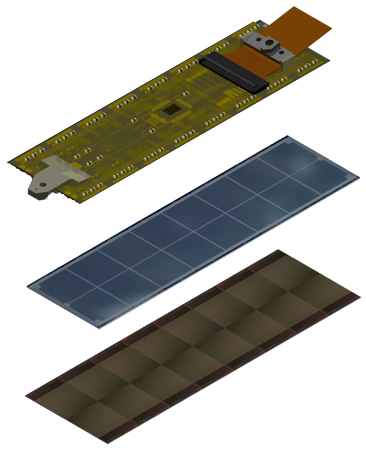
\includegraphics[width=0.33\textwidth]{pixel/fpix_structure1}
  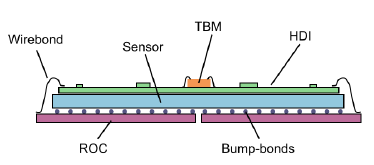
\includegraphics[width=0.63\textwidth]{pixel/fpix_structure2}
  \caption[FPix module structure.]{FPix module structure; The bare silicon sensor is bump-bonded to the ROCs to form the BBM; then the HDI is glued on top of the BBM and wirebonded to the ROCs.}\label{fig:fpix_struc}
\end{figure}

The current CMS pixel detector is composed of 1184 pixel modules in the BPIX sector with a total 79 million of pixels; the FPix sector contains 672 with approximately 45 million of pixels. Figure \ref{fig:fpix_struc} shows an schematic view of the FPix modules structure. The n$^{+}$-in-n \ti{Silicon sensor} is Bump-Bonded to the 16 ROC to form the detector unit known as \ti{Bump-Bonded Module} (BBM) with 66560 pixels. The \ti{High Density Interconnect} (HDI) is glued on top of the BBM and wirebonded to the ROCs to provide them the required signals and power. The modules are attached to the support structure using the end holders glued to the HDI.

\section{FPix module assembly}

The construction of the modules for the current FPix system was divided between two sites located at Purdue University and UNL; testing facilities were located at University of Kansas and Fermi National Accelerator Laboratory (Fermilab). The integration facility was based at Fermilab. 

The BBM was prepared by a commercial vendor, while the HDI was populated at Fermilab, with all the electronic components like resistors, capacitors and the central component known as \ti{Token Bit Manager} (TBM) which is in charge of managing the information coming from the silicon sensors and going to the ROCs. Both BBM and HDI were sent to the assembly sites ready to be glued together.  


\begin{figure}[!h]
  \centering
  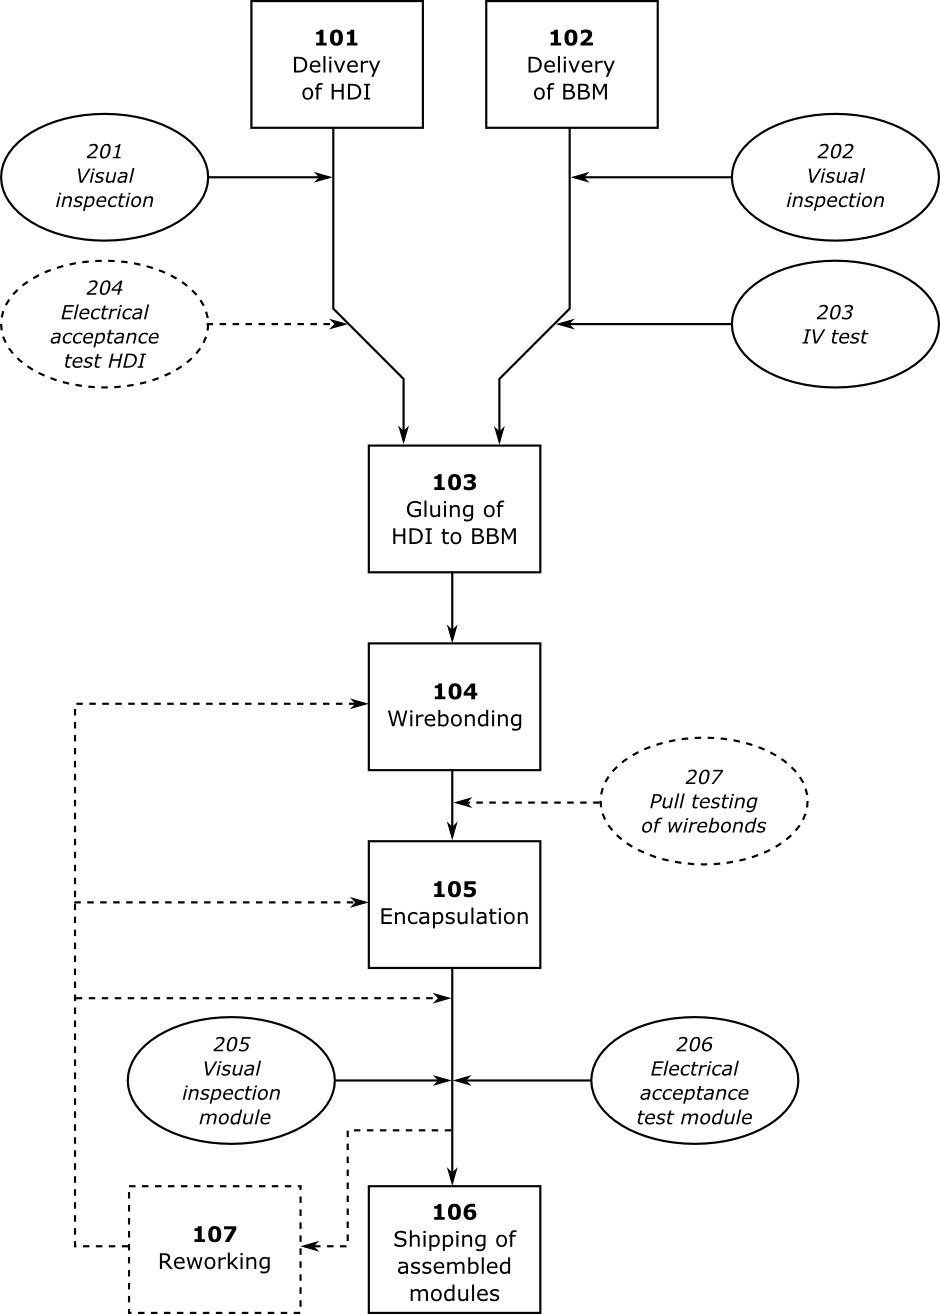
\includegraphics[width=0.7\textwidth]{pixel/UNLworkflow}
  \caption[UNL module assembly work flow.]{UNL module assembly work flow. Dashed lines represent occasional quality testing and reworking procedures; 10X numbers represent the stage within the assembly procedure while 20X numbers represent testing stages along the assembly procedure.}\label{fig:unlworkflow}
\end{figure}


The module production procedure was designed following a production line structure. Figure \ref{fig:unlworkflow} shows the work flow followed at the UNL assembly site. Once the BBM and HDI arrive, they are
submitted to visual inspection looking for defects, scratches, dents or short circuits. The modules passing the visual inspection are tested for electrical acceptance and performance. BBM and HDI are then glued employing robotic pick-and-place machines that integrate optic tools, pattern recognition algorithms, and glue dispensing; the semi-automated gluing process improves the uniformity of the technique. After 10 hours of curing, modules are moved to the wirebonding station where ROCs and HDI are electrically connected employing semi-automated ultrasonic wirebongding machines; occasionally, some of the wires are pull tested for quality control. In the next stage, the wirebonds are encapsulated with an elastomeric compound in order to protect them against mechanical damage and electrical shorts; the encapsulation process is performed employing the robotic pick-and-place machine which also integrates the encapsulant dispensing system.

The module assembly sites were also responsible for the testing and characterization of the assembled pixel modules. That testing included, visual inspection, electrical acceptance and performance testing; in case of any necessary reworking, the modules were returned to the appropriate stage. In the final stage, the assembled and tested modules were shipped to University of Kansas for further characterization.  

Each stage in the assembly procedure is documented with an ~\ti{Standard Operating Procedure} (SOP) document that describes the procedures to be followed by the operator. The full set of SOPs can be found in Reference \cite{unl_sop}.     


In the following sections a detailed description of the gluing and encapsulation stages will be presented. 




















































%% \begin{figure}[!h]
%%   \centering
%%   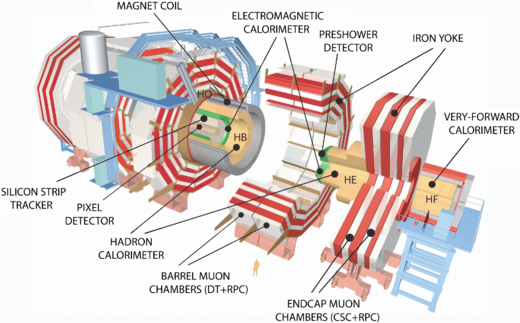
\includegraphics[scale=0.25]{cms}
%%   \caption {ref:  }\label{cms}
%% \end{figure}



\subsection{The Gluing stage}


The module assembly sequence begins by manually placing pre-tested, known good 2 x 8 BBMs and HDI
on vacuum chucks on the baseplate of the pick-and-place machine.


The machine program successively moves the camera (fixed to the machine motion head) to view the fiducial on the BBM sensors and HDI components and acquires the fiducial location using pattern recognition,
picks up a dispensing tool from a the tool rack and dispenses epoxy on the sensors, returns the dispensing tool to the tool rack, picks up a vacuum tool from the tool rack to pick-and-place individual HDI onto sensors (making adjustments based on the actual part locations in the machine to accurately align and join the components), and returns the vacuum tool to the tool rack. Module end holders are also aligned and glued to the modules using custom tooling and the pick-and-place machine. Following mechanical assembly, HDI are wirebonded to the ROCs using semi-automated ul-
trasonic wirebonding machines. Routine pull tests of sample wirebonds will be performed
for quality control. The wirebonds will be encapsulated with an elastomeric compound using
semi-automated dispensing equipment. The module assembly sites will also be responsible for
the testing and characterization of the assembled pixel modules. Modules will be thermally
cycled within the operating temperature range (-20 ◦ C to 20 ◦ C) while monitoring ROC digital
and analog currents. Modules which pass the acceptance criteria will then be assembled onto
the half-disk blades.

The module assembly and testing schedule will depend on the throughput of the pixel modules delivered from the bump-bonding vendors to the module
assembly sites.




%% \begin{figure}[!h]
%%   \centering
%%   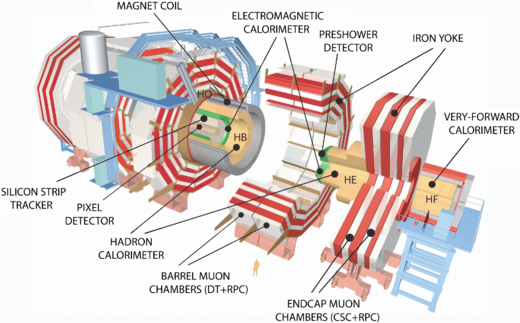
\includegraphics[scale=0.25]{cms}
%%   \caption {ref:  }\label{cms}
%% \end{figure}

\subsection{The Encapsulation stage}

%% \begin{figure}[!h]
%%   \centering
%%   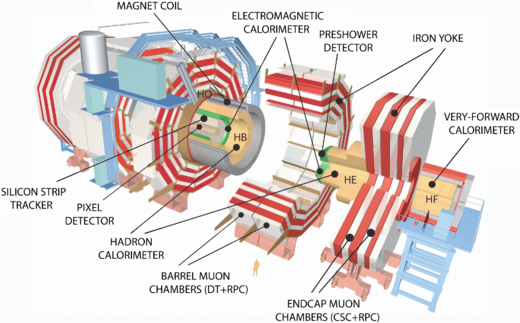
\includegraphics[scale=0.25]{cms}
%%   \caption {ref:  }\label{cms}
%% \end{figure}

\subsection{The FPix module production yields}

%% \begin{figure}[!h]
%%   \centering
%%   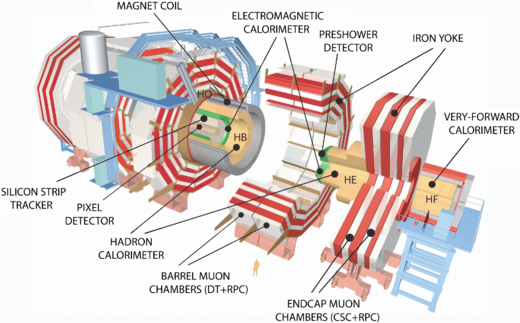
\includegraphics[scale=0.25]{cms}
%%   \caption {ref:  }\label{cms}
%% \end{figure}
